%%
%% This is file `sample-xelatex.tex',
%% generated with the docstrip utility.
%%
%% The original source files were:
%%
%% samples.dtx  (with options: `sigconf')
%% 
%% IMPORTANT NOTICE:
%% 
%% For the copyright see the source file.
%% 
%% Any modified versions of this file must be renamed
%% with new filenames distinct from sample-xelatex.tex.
%% 
%% For distribution of the original source see the terms
%% for copying and modification in the file samples.dtx.
%% 
%% This generated file may be distributed as long as the
%% original source files, as listed above, are part of the
%% same distribution. (The sources need not necessarily be
%% in the same archive or directory.)
%%
%% The first command in your LaTeX source must be the \documentclass command.
\documentclass[sigconf]{acmart}
\usepackage{algorithm}
\usepackage{algpseudocode}
\usepackage{amsmath}
\usepackage{listings}
\usepackage{xcolor}

\lstset{
  language=Java,
  basicstyle=\ttfamily\small,
  keywordstyle=\color{blue},
  commentstyle=\color{gray},
  stringstyle=\color{red},
  numbers=left,
  numberstyle=\tiny\color{gray},
  stepnumber=1,
  numbersep=5pt,
  backgroundcolor=\color{white},
  showspaces=false,
  showstringspaces=false,
  showtabs=false,
  frame=single,
  tabsize=2,
  captionpos=b,
  breaklines=true,
  breakatwhitespace=false,
  escapeinside={\%*}{*)}
}

%%
%% \BibTeX command to typeset BibTeX logo in the docs
\AtBeginDocument{%
  \providecommand\BibTeX{{%
    \normalfont B\kern-0.5em{\scshape i\kern-0.25em b}\kern-0.8em\TeX}}}

%% Rights management information.  This information is sent to you
%% when you complete the rights form.  These commands have SAMPLE
%% values in them; it is your responsibility as an author to replace
%% the commands and values with those provided to you when you
%% complete the rights form.

%%
%% Submission ID.
%% Use this when submitting an article to a sponsored event. You'll
%% receive a unique submission ID from the organizers
%% of the event, and this ID should be used as the parameter to this command.
%%\acmSubmissionID{123-A56-BU3}

%%
%% The majority of ACM publications use numbered citations and
%% references.  The command \citestyle{authoryear} switches to the
%% "author year" style.
%%
%% If you are preparing content for an event
%% sponsored by ACM SIGGRAPH, you must use the "author year" style of
%% citations and references.
%% Uncommenting
%% the next command will enable that style.
%%\citestyle{acmauthoryear}

%%
%% end of the preamble, start of the body of the document source.
\begin{document}

%%
%% The "title" command has an optional parameter,
%% allowing the author to define a "short title" to be used in page headers.
\title{Mandelbrot Set}

%%
%% The "author" command and its associated commands are used to define
%% the authors and their affiliations.
%% Of note is the shared affiliation of the first two authors, and the
%% "authornote" and "authornotemark" commands
%% used to denote shared contribution to the research.
% \author{Ben Trovato}
% \authornote{Both authors contributed equally to this research.}
% \email{trovato@corporation.com}
% \orcid{1234-5678-9012}
% \author{G.K.M. Tobin}
% \authornotemark[1]
% \email{webmaster@marysville-ohio.com}
% \affiliation{%
%   \institution{Institute for Clarity in Documentation}
%   \streetaddress{P.O. Box 1212}
%   \city{Dublin}
%   \state{Ohio}
%   \postcode{43017-6221}
% }

\author{Branko Petrevski}
\affiliation{%
  \institution{FAMNIT}
  \city{Koper}
  \country{Slovenia}}
\email{89221032@student.upr.si}

%%
%% By default, the full list of authors will be used in the page
%% headers. Often, this list is too long, and will overlap
%% other information printed in the page headers. This command allows
%% the author to define a more concise list
%% of authors' names for this purpose.
\renewcommand{\shortauthors}{Branko Petrevski}

%%
%% The abstract is a short summary of the work to be presented in the
%% article.
\begin{abstract}
  In this \LaTeX\ paper is presented plotting of the mandelbrot set in the programming language Java using the set of graphics packages JavaFX. It contains the options panning and zooming on the canvas as well as saving an image of the current view-port with custom dimensions. The Java program works in sequential, parallel and distributive mode. The parallel part divides the image in even parts among the current number of threads and uses CyclicBarrier to await all threads to finish their computation before updating the fractal canvas.
\end{abstract}

%% A "teaser" image appears between the author and affiliation
%% information and the body of the document, and typically spans the
%% page.
\begin{teaserfigure}
  \includegraphics[width=\textwidth]{mandelbrot.png}
  \caption{Representation of the mandelbrot set.}
  \Description{Mandelbrot set at its finest.}
  \label{fig:teaser}
\end{teaserfigure}

%%
%% This command processes the author and affiliation and title
%% information and builds the first part of the formatted document.
\maketitle

\section{Introduction}
The Mandelbrot set is a mesmerizing and complex mathematical idea which has captivated the interest of mathematicians, scientists as well as artists. At a very fundamental level, the Mandelbrot set is an example of what we call a fractal. That means it possesses self-similarity at all scales. In order to understand how it is built, we need to explore the land of complex numbers: an extension (beyond) our traditional number line where now there exists a dimension called imaginary. The Mandelbrot set is generated by iterating a super simple little formula, plugging in complex numbers over and over again to see what happens. 
complex numbers \( c \) for which 
\[
f_c(z) = z^2 + c
\]
may not diverge when iterated from \( z = 0 \). More explicitly, 
\[
\left\{ f_c^n(z) \right\}_{n \in \mathbb{N}}
\]
is pointwise-bounded in absolute value; here we define 
\[
f_c^0(z) = z \quad \text{and} \quad f_c^{n+1}(z) = f_c(f_c^n(z)).
\]

The color version yiels a graphical representation of the set: to every point c in the plane is assigned an appropriate colour depending on does (and how fast) sequence fn converges. That is, rendering pixel (i,j) if they correspond to a complex number c by escape time processing algorithm.

\begin{algorithm}[H] % H to fix the position
\caption{Compute Pixel}
\begin{algorithmic}[1]
\Procedure{ComputePixel}{$cX, cY$}
    \State $zy \gets 0$
    \State $zx \gets 0$
    \State $iter \gets 0$
    \While{$iter < maxIter$ \textbf{and} $zx^2 + zy^2 < 4$}
        \State $tmp \gets zx^2 - zy^2 + cX$
        \State $zy \gets 2.0 \times zx \times zy + cY$
        \State $zx \gets tmp$
        \State $iter \gets iter + 1$
    \EndWhile
    \State \textbf{return} $iter$
\EndProcedure
\end{algorithmic}
\end{algorithm}

The \texttt{computePixel} method calculates the number of iterations required for a point in the complex plane to escape the Mandelbrot set's boundary. It initializes the complex number components \texttt{zx} and \texttt{zy} to zero and iteratively updates them using the formula \texttt{zx = zx * zx - zy * zy + cX} and \texttt{zy = 2.0 * zx * zy + cY} until the magnitude exceeds 4 or the maximum number of iterations is reached. The method returns the iteration count, which is used to determine the color of the pixel.
Since every pixel is calculated independently, the algorithm naturally allows for parallelisation. It can be easily adapted in a threaded, process or distributed way on several machines. The following sections of this paper will describe the parallelization approaches we used and provide performance results with different levels of procs.


\section{Design Overview}
The program aims to draw the Mandelbrot set in Java using JavaFX for GUI and rendering. This program generates the fractal image in an optimized manner using both sequential and parallel computation. Main class that will initialize the JavaFX application, setup canvas for rendering and manage Zooming/Panning of drawing.
\\\\
In this non-parallel approach, we implemented a regular sequential computation that iterates over all pixels on the canvas and computes the corresponding point in complex plane for them one by one to then use escape time algorithm to color each pixel. They describe this method because of how easy it is to implement, which makes it practical for low iteration counts or images that are not too big. Its biggest weakness is that it is single-threaded and therefore slow for large images or high iteration counts.
\\\\
The parallel computing solution divides the canvas into pieces that are worked on by different threads and supports synchronization via a `CyclicBarrier` mechanism to properly update the information when all thread have done their jobs. In this way, the computation is accelerated by multi-core processors and works faster for a large number of images or iterations. As a trade-off, they result in more complex implementations and have various thread synchronization issues.
\\\\
The `computePixel` method, which states the escape time algorithm, applies Mandelbrot formula in a loop to understand how fast points are running from a certain boundary. Number of iterations is used to determine the color at each pixel and its calculated in calculateColor method. This allows us to use some optimization techniques like looking up if a point is inside either the main cardioid or period-2 bulb, so we can quickly skip it and not waste time computing an orbit. This value provide optimal balance between how accurate the fractal result later, and performance in generation it.

\begin{algorithm}
\caption{Main Algorithm}
\begin{algorithmic}[1]
\State Initialize screen, iterations, zoom, positions
\State Parse arguments for width, height, mode
\If{distributive mode}
    \State Initialize MPI
    \If{MPI rank is 0}
        \State Print settings
    \EndIf
\Else
    \State Print settings
\EndIf
\State Initialize pixel array
\State Execute mode (sequential, parallel, distributive)
\State Print commands
\While{input is not 'q'}
    \State Read input
    \For{each command}
        \If{empty or computing}
            \State Continue
        \EndIf
        \State Handle command
        \State Start computation
        \State Print state
        \State Execute computation
        \State Finish computation
    \EndFor
\EndWhile
\If{distributive mode}
    \State Finalize MPI
\EndIf
\end{algorithmic}
\end{algorithm}

\section{Problem description}

 We will first discuss the issues that the CyclicBarrier and MPI interfaces are intended to address before going over how they are implemented. To achieve that, we will outline the precise actions that each of the program's four execution modes should take.

\begin{itemize}
    \item \textbf{Sequential mode}: The following mode uses a single thread to execute all the necessary calculations and operations. First, it loads the width and height arguments and based on them initializes the application, canvas creation, and starts calculating pixels to display the Mandelbrot set. It is slower for bigger dimensions and a higher number of iterations.
    \item \textbf{Parallel mode}: In this mode, we divide the computational work of the previous method into a new method among a specified number of threads, which take care of an equal part of the fractal computation and return the results on the canvas as soon as all of them are done. Then the canvas updates the image.
    \item \textbf{Distributive mode}: Same as parallel but instead of threads, we are using MPI to distribute the work among different nodes in a cluster. The results are then sent back to the main node and the canvas updates the image.
\end{itemize}

\section{CyclicBarrier and Threads}

In addition to specifying the {\itshape problem description} to be used in
In the Mandelbrot project, a \texttt{CyclicBarrier} is used to synchronize multiple threads during the parallel computation of the fractal. Each thread processes a distinct chunk of the canvas, computing the Mandelbrot set for its assigned section. The \texttt{CyclicBarrier} ensures that all threads complete their computations before updating the canvas with the results. This approach leverages multi-core processors to significantly speed up the rendering process compared to a single-threaded implementation. By dividing the workload among threads and synchronizing them with a \texttt{CyclicBarrier}, the project achieves efficient and concurrent computation, enhancing performance for large images and high iteration counts.

The \texttt{CyclicBarrier} is initialized with the number of threads and a barrier action that updates the canvas. Each thread computes its chunk and calls the \texttt{await} method on the barrier, blocking until all threads reach the barrier. Once all threads have called \texttt{await}, the barrier action is executed, updating the canvas with the computed image. This method ensures that the canvas is only updated once all threads have finished their computations, maintaining synchronization and improving performance.
\\
In Java, a thread is a lightweight process that allows concurrent execution of code. Threads are essential for performing multiple tasks simultaneously within a program, improving performance and responsiveness. Java provides the \texttt{Thread} class and the \texttt{Runnable} interface to create and manage threads.

To create a thread, you can either extend the \texttt{Thread} class and override its \texttt{run} method or implement the \texttt{Runnable} interface and pass an instance of it to a \texttt{Thread} object. The \texttt{start} method is called to begin the execution of the thread, which internally calls the \texttt{run} method.
\\
These parts are implemented in the method computeParallel as follows:
\begin{lstlisting}
private void computeParallel() {

    long t0 = System.currentTimeMillis();

    this.barrier = new CyclicBarrier(cores, () -> {
        isComputing = false;
    });

    this.writableImage = new WritableImage((int) DEFAULT_SCREEN_WIDTH, (int) DEFAULT_SCREEN_HEIGHT);
    this.pixelWriter = writableImage.getPixelWriter();

    int chunkSize = (int) DEFAULT_SCREEN_HEIGHT / cores;

    for (int i = 0; i < cores; i++) {
        int startRow = i * chunkSize;
        int endRow = (i == cores - 1) ? (int) DEFAULT_SCREEN_HEIGHT : startRow + chunkSize;
        new Thread(new MTask(i,
                startRow,
                endRow,
                barrier,
                (int) DEFAULT_SCREEN_HEIGHT,
                (int) DEFAULT_SCREEN_WIDTH,
                cores,
                xPos,
                yPos,
                zoom,
                maxIter,
                writableImage,
                pixelWriter,
                graphicsContext)).start();
    }

    // Wait for all tasks to finish
    try {
        barrier.await();
        System.out.println("All threads have reached the barrier. Barrier action executed.");
    } catch (Exception e) {
        e.printStackTrace();
    }
    // Output computation time
    System.out.println("Parallel time: " + (System.currentTimeMillis() - t0) + "ms ");
    isComputing = false;
}
\end{lstlisting}

\section{Technical Remarks}
The program was written in Java with some helper libraries to implement it. Certain aspects of the project rely on JavaFX features for rendering Mandelbrot set and user interactions, written purely as an academic exercise in order to get familiar with a lightweight tool bundled into recent versions of JVM. The program is further intended to be highly portable, and can run on any instance of the Windows or Linux operating system that has a JRE version which recent enough. The rest of the program configuration (including job specification) is loaded from command line parameters and we just write output to a PNG image because it is the most widely supported image format by mainstream image viewer. More technical details are in the subsections below.

\subsection{Thread Synchronization}
The use of \texttt{CyclicBarrier} ensures that all threads complete their computations before updating the canvas. This synchronization mechanism is crucial for maintaining consistency in the rendered image.

\subsection{Parallel Computation}
By dividing the canvas into chunks and assigning each chunk to a separate thread, the program leverages multi-core processors to speed up the Mandelbrot set computation. This parallel approach significantly reduces the computation time compared to a single-threaded implementation.

\subsection{Dynamic Thread Management}
The number of threads is dynamically set to the number of available processors (\texttt{Runtime.getRuntime().availableProcessors()}). This ensures optimal utilization of system resources.

\subsection{Barrier Action}
The barrier action updates the canvas with the computed image once all threads have reached the barrier. This ensures that the canvas is only updated when all computations are complete, preventing partial updates.

\subsection{Error Handling}
The code includes error handling for \texttt{InterruptedException} and \texttt{BrokenBarrierException} during the barrier synchronization, ensuring that any issues during thread execution are properly managed.

\subsection{Zoom and Navigation}
The \texttt{handleKeyPress} method allows for interactive zooming and navigation of the Mandelbrot set. This enhances the user experience by providing real-time feedback on the fractal exploration.

\subsection{Color Calculation}
The \texttt{calculateColor} method generates colors based on the iteration count, creating a visually appealing representation of the Mandelbrot set. Points inside the set are colored black, while points outside are colored based on their escape time.

\subsection{Sequential and Parallel Modes}
The program supports both sequential and parallel computation modes, allowing for performance comparison and flexibility in execution.

\subsection{Canvas Resizing and Saving}
The \texttt{saveImage} method allows users to save the fractal image as a PNG file with user-specified dimensions. This feature is useful for exporting high-resolution images of the fractal.

\subsection{JavaFX Integration}
The use of JavaFX for the graphical user interface provides a modern and responsive platform for rendering the Mandelbrot set and handling user interactions.

\section{Results}

The tests were run on 4 core processor Intel i5 - 8300H with 8 threads for maximum number of iterations 2000 and for input string
\begin{minipage}[t]{\columnwidth}
\textit{"++++++++aaaaaaa++++++++++ssssssssss++++++++++++++awwww+
\\+++++++++++d--ssswwwwwwwwwwwww+++++++++++++++++++"}
\end{minipage}. Parameters that were varied was the width and height of the Mandelbrot canvas and were the following: 1000x1000, 2000x2000, 3000x3000 px. For each triple of parameters, the program was executed 7 times and the given results are the averages of those 7 times execution for every mode, sequential, parallel with 8 threads and distributive with 8 nodes. As we can see in the first graph, it illustrates the computation times for zooming and panning the Mandelbrot set with dimensions 1000x1000 using three different modes: sequential, parallel, and distributive. The x-axis represents different iterations, while the y-axis indicates the computation time in milliseconds. The sequential mode, represented by the blue line, consistently shows the highest computation times, peaking around 400 milliseconds at certain points. The parallel mode, depicted by the orange line, demonstrates significantly lower computation times compared to the sequential mode, maintaining a relatively stable performance with minor fluctuations. The distributive mode, shown by the green line, exhibits the lowest computation times overall, with a noticeable reduction in computation time as the iterations progress. Both parallel and distributive modes show a significant drop in computation time towards the end of the iterations, converging to minimal values. This analysis highlights the efficiency of parallel and distributive computing in reducing computation times for complex tasks like generating the Mandelbrot set. We can see similar for the second and third graph.

\begin{figure}[H]
    \centering
    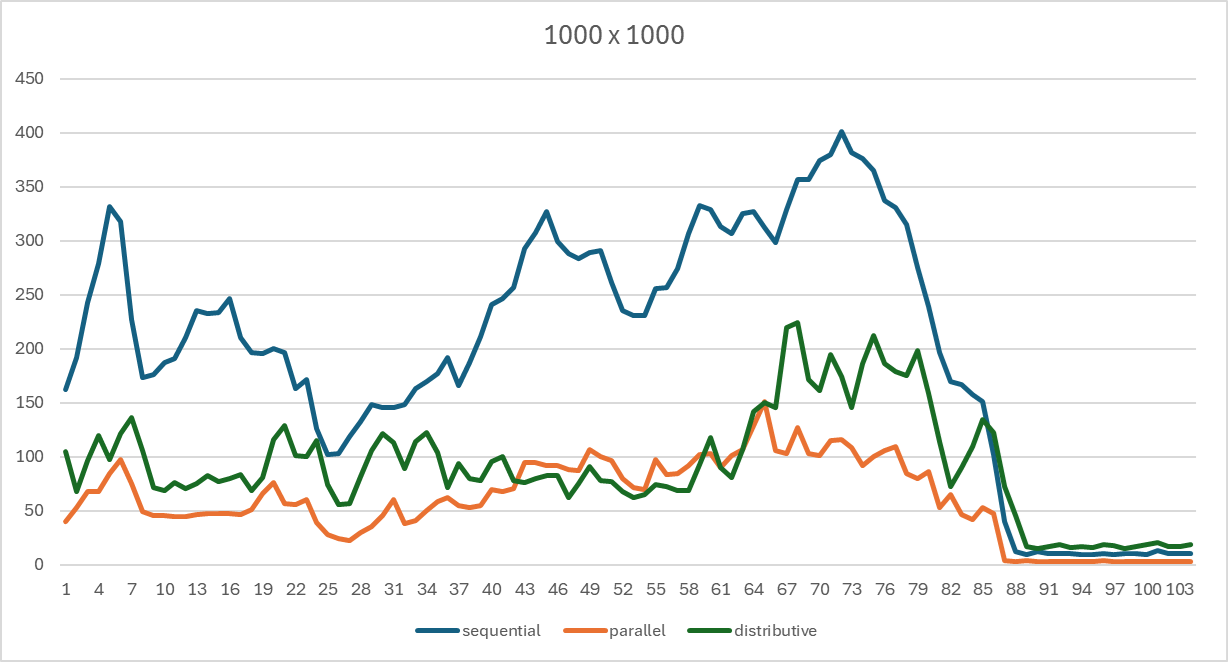
\includegraphics[width=0.5\textwidth]{Mandelbrot 1000x1000.png} % Replace 'example-image' with your image file name
    \caption{Speedup for width and height 1000}
    \label{fig:1000}
\end{figure}

\begin{figure}[H]
    \centering
    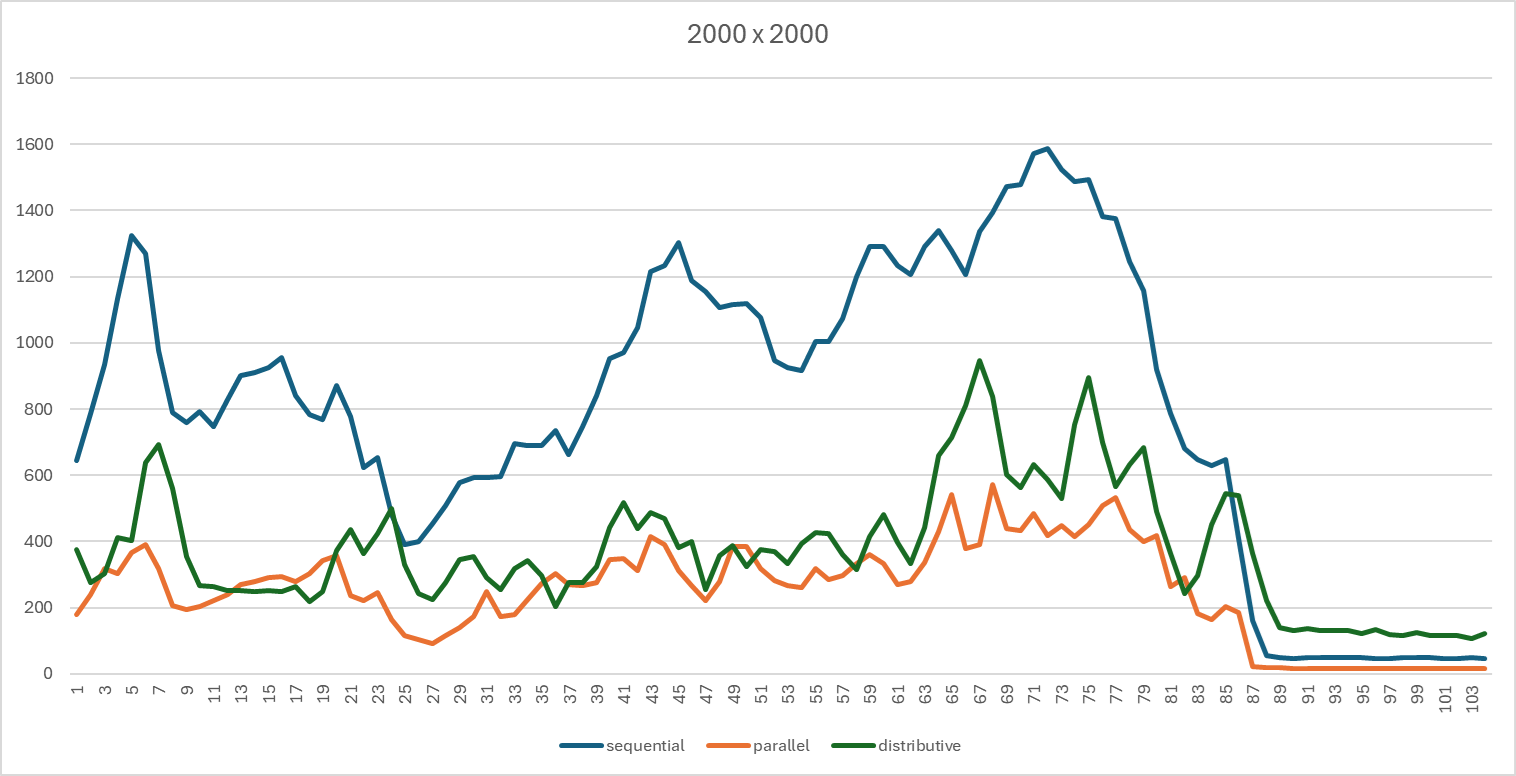
\includegraphics[width=0.5\textwidth]{Mandelbrot 2000x2000.png} % Replace 'example-image' with your image file name
    \caption{Speedup for width and height 2000}
    \label{fig:2000}
\end{figure}

\begin{figure}[H]
    \centering
    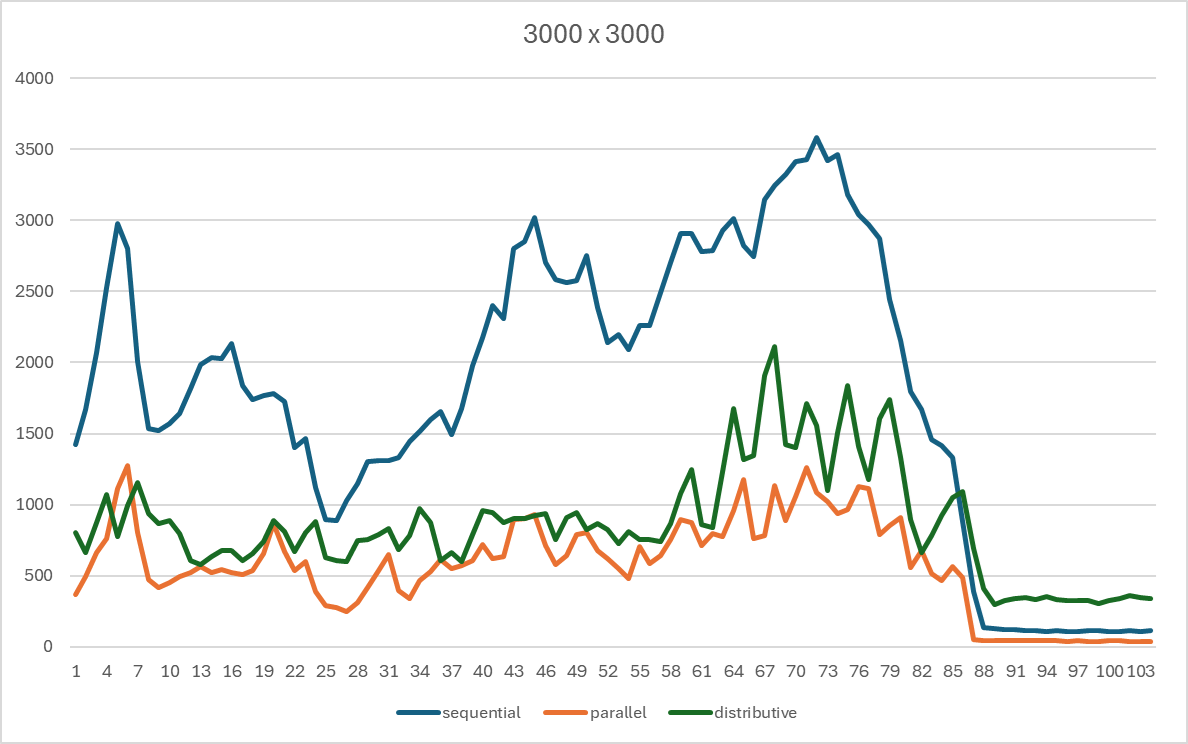
\includegraphics[width=0.5\textwidth]{Mandelbrot 3000x3000.png} % Replace 'example-image' with your image file name
    \caption{Speedup for width and height 3000}
    \label{fig:3000}
\end{figure}

\section{Conclusion}
In conclusion, tests on a 4-core Intel i5-8300H with 8 threads and up to 2000 iterations reveal significant performance gains from parallel and distributed computing in Mandelbrot set generation. Parallel processing with Java threads and CyclicBarrier, and distributed computing with MPI, notably reduced computation times compared to the sequential approach.

For canvas sizes of 1000x1000, 2000x2000, and 3000x3000 pixels, parallel computing consistently outperformed sequential processing, while distributed computing achieved the best efficiency. Sequential times peaked at around 400 milliseconds, whereas parallel times were lower and stable, and distributed times were the fastest. Both parallel and distributed methods also showed reduced computation times as iterations increased.

These results highlight the effectiveness of parallel and distributed computing techniques in optimizing performance for complex tasks like Mandelbrot set rendering.


\end{document}
\endinput
%%
%% End of file `sample-xelatex.tex'.
